\newpage
\section{Auswertung}
\label{sec:Auswertung}

\begin{table}
  \centering
  \caption{Temperatur und Druck bei Verdampfung des Wassers. Der Druck hat eine Messunsicherheit von
  $\pm$mB, die Temperatur von $\pm 1$ K.},
  \label{tab:Messreihe_1}
\begin{tabular}{
  c c||c c||c c||c c
}
\toprule 
$T/ \unit{\kelvin}$ & $p / \text{mB}$ & $T/ \unit{\kelvin}$ & $p / \text{mB}$&
$T/ \unit{\kelvin}$ & $p / \text{mB}$ & $T/ \unit{\kelvin}$ & $p / \text{mB}$ \\
\midrule
293,15  & 40   & 313,15  & 372  & 333,15  & 528  & 353,15  & 773 \\
294,15  & 167  & 314,15  & 379  & 334,15  & 537  & 354,15  & 790 \\
295,15  & 228  & 315,15  & 385  & 335,15  & 549  & 355,15  & 810 \\
296,15  & 255  & 316,15  & 395  & 336,15  & 562  & 356,15  & 826 \\
297,15  & 274  & 317,15  & 400  & 337,15  & 571  & 357,15  & 844 \\
298,15  & 287  & 318,15  & 405  & 338,15  & 578  & 358,15  & 856 \\
299,15  & 296  & 319,15  & 412  & 339,15  & 586  & 359,15  & 879 \\
300,15  & 303  & 320,15  & 421  & 340,15  & 600  & 360,15  & 901 \\
301,15  & 310  & 321,15  & 431  & 341,15  & \text{--}  & 361,15  & 913 \\
302,15  & 316  & 322,15  & 439  & 342,15  & 628  & 362,15  & 933 \\
303,15  & 322  & 323,15  & 445  & 343,15  & 638  & 363,15  & 944 \\
304,15  & 327  & 324,15  & 453  & 344,15  & 650  & 364,15  & 966 \\
305,15  & 331  & 325,15  & 461  & 345,15  & 660  & 365,15  & 979 \\
306,15  & 336  & 326,15  & 465  & 346,15  & 670  & 366,15  & 990 \\
307,15  & 341  & 327,15  & 476  & 347,15  & 690  & 367,15  & 1015\\
308,15  & 347  & 328,15  & 482  & 348,15  & 701  & 368,15  & 1030\\
309,15  & 351  & 329,15  & 491  & 349,15  & 716  & 369,15  & 1046\\
310,15  & 356  & 330,15  & 500  & 350,15  & 723  & 370,15  & 1061\\
311,15  & 362  & 331,15  & 511  & 351,15  & 743  & 371,15  & 1079\\
312,15  & 367  & 332,15  & 520  & 352,15  & 760  & 372,15  & 1093\\
      &   &       &       &       &      & 373,15  & 1108 \\
\bottomrule
\end{tabular}
\end{table}
\begin{table}
  \centering
  \caption{Temperatur und Druck bei Verdampfung des Wassers für $p\geq 1$.Der Druck hat eine Messunsicherheit von
  $\pm$mB, die Temperatur von $\pm 1$ K.},
  \label{tab:Messreihe_2}
\begin{tabular}{
  c c||c c
}
\toprule 
$p$/B & $T$/K & $p$/B & $T$/K\\
\midrule
1000  & 391,15 & 9000  & 447,15\\
2000  & 404,15 & 10000 & 451,15\\
3000  & 413,15 & 11000 & 454,15\\
4000  & 419,15 & 12000 & 459,15\\
5000  & 427,15 & 13000 & 461,15\\
6000  & 433,15 & 14000 & 463,15\\
7000  & 438,15 & 15000 & 465,15\\
8000  & 443,15 &       &       \\
\bottomrule
\end{tabular}
\end{table}

Mit diesen Messwerten lassen sich folgende Grafiken erstellen:
\begin{figure}
  \begin{subfigure}{0.48\textwidth}

    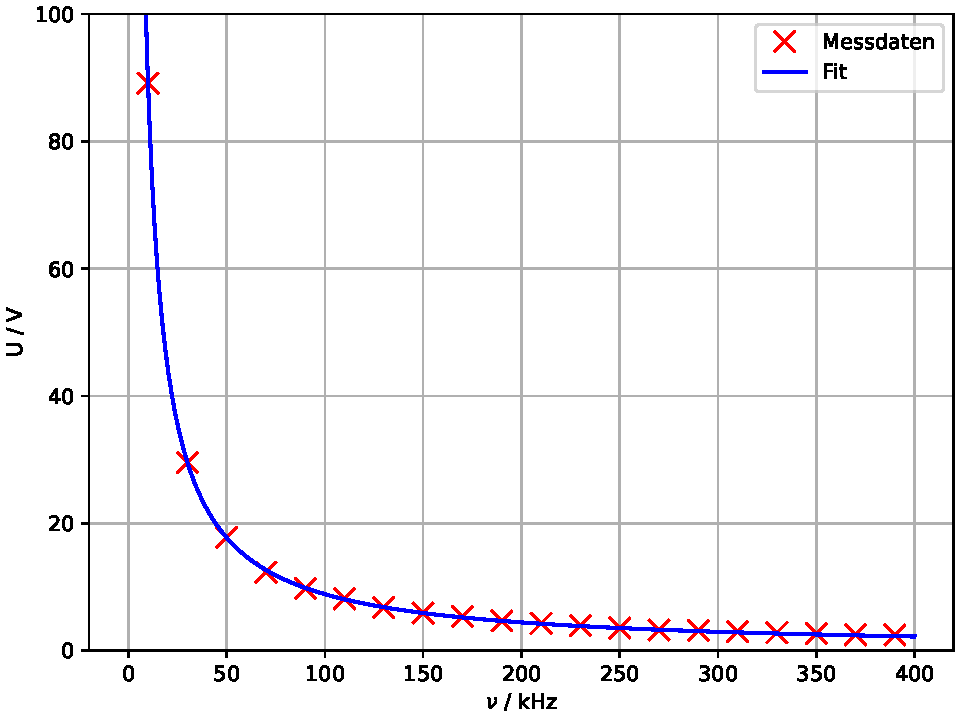
\includegraphics{python/plota}
    \caption{Messwerte für den Bereich von $30$ bis $1000 mbar$}
    \label{fig:MesswerteKlein}
  \end{subfigure}
  \hfill
  \begin{subfigure}
    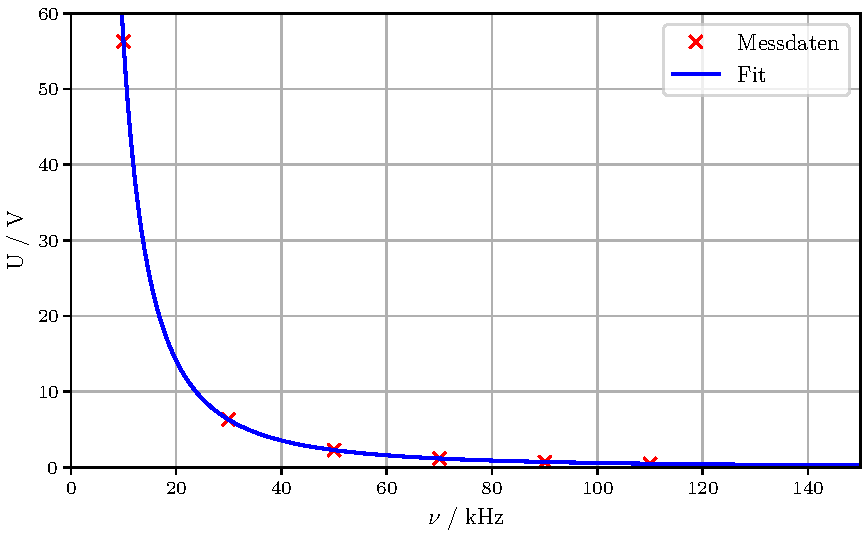
\includegraphics{python/plotb}
    \caption{Messwerte für den Bereich von $1$ bis $15 bar$}
    \label{fig:MesswerteGross}
  \end{subfigure}
  \caption{Die Messwerte der ersten Messreihe aufgetragen als der Logarithmus des Drucks $p$
  gegen die reziproke absolute Temperatur $T$.}
  \label{fig:Teila}
\end{figure}
Um hier raus die Verdampfungswärme von Wasser zu bestimmen, legt man eine Gerade durch die Messwerte.
Diese wird mittels Python für den Bereich von $30$ bis $1000 mbar$ erstellt und sieht folgendermaßen aus:
\begin{figure}
  \centering
  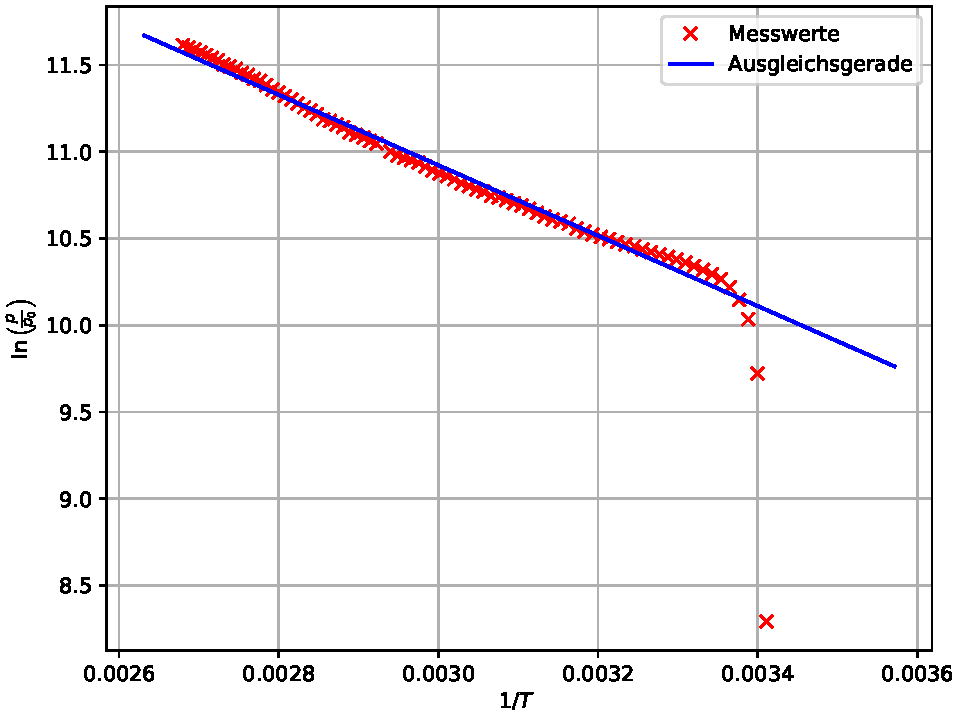
\includegraphics[width=\textwidth]{python/plotc}
  \caption{Die Messwerte der zweiten Messreihe aufgetragen als der Logarithmus des Drucks $p$
  gegen die reziproke absolute Temperatur $T$.}
\end{figure}
Für diesen Fit wurden die ersten zwei Messwerte dieser Reihe nicht berücksichtigt, da diese aus der Reihe rausspringen.
Für die Verdampfungswärme von Wasser ergibt sich:
\begin{*equation}
  L = 2029.10266825 \pm 20.99148783
\end{*equation}
L beschreibt die Steigung der Ausgleichsgeraden.


\\
Die allgemeine Gasgleichung ist pV=RT. 
% Siehe \autoref{fig:plot} und \autoref{tab:tabelle}!
